\documentclass[tikz]{standalone}

\usepackage{tikz}
\usetikzlibrary{quotes}
%\usepackage{}
%\use...library{}

%\tikzset{every figure} = []
\begin{document}
	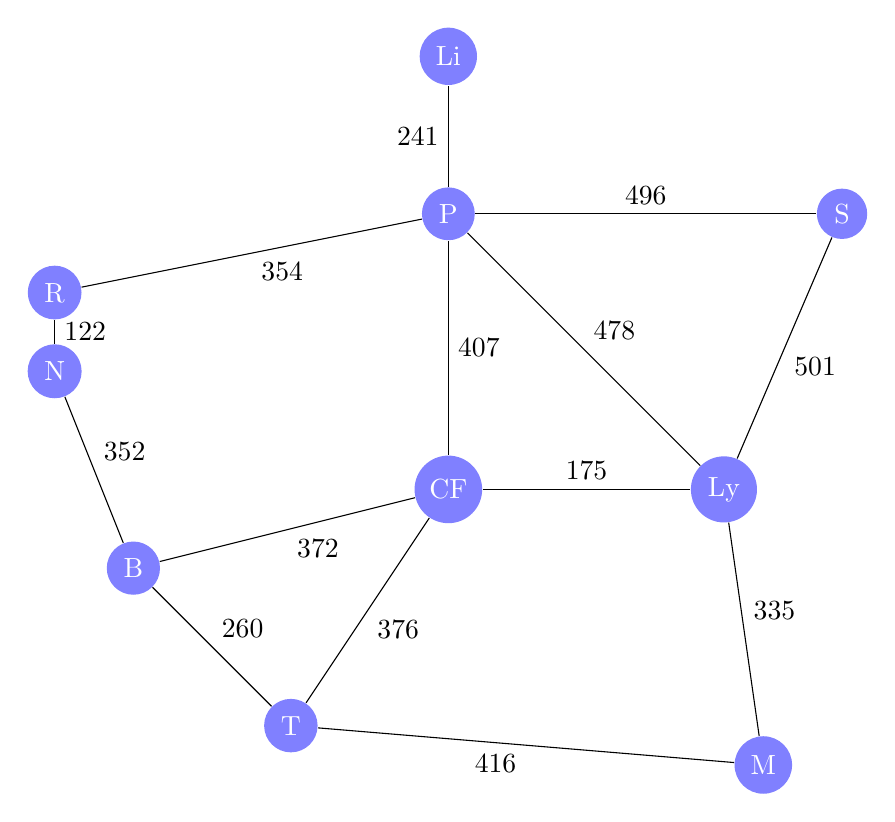
\begin{tikzpicture} 
		%\node (nom node) at(x,y) [options separées par virgules] {affichage} ;
		\node (node 1) at(0,8) [circle,double, double distance =1.2pt,text=white,fill=blue!50,] {P} ;
		\node (node 2) at(0,10) [circle,double, double distance =1.2pt,text=white,fill=blue!50,] {Li} ;
		\node (node 3) at(5,8) [circle,double, double distance =1.2pt,text=white,fill=blue!50,] {S} ;
		\node (node 4) at(-5,7) [circle,double, double distance =1.2pt,text=white,fill=blue!50,] {R} ;
		\node (node 5) at(0,4.5) [circle,double, double distance =1.2pt,text=white,fill=blue!50,] {CF} ;
		\node (node 6) at(3.5,4.5) [circle,double, double distance =1.2pt,text=white,fill=blue!50,] {Ly} ;
		\node (node 7) at(4,1) [circle,double, double distance =1.2pt,text=white,fill=blue!50,] {M} ;
		\node (node 8) at(-5,6) [circle,double, double distance =1.2pt,text=white,fill=blue!50,] {N} ;
		\node (node 9) at(-4, 3.5) [circle,double, double distance =1.2pt,text=white,fill=blue!50,] {B} ;
		\node (node 10) at(-2,1.5) [circle,double, double distance =1.2pt,text=white,fill=blue!50,] {T} ;
		
%(nom node): charactères interdits: ) [ ;
%at(x,y): optionel : x et y doivent être des coordonnées viables: des nombres 
%[options séparées par virgules]:  les options du nœud. En détail certain: 			 
	%fill=couleur
	%label=texte du label ou label={texte du label} ou label={:texte du label}
	%label={position du label:texte du label}
	%label={[couleur du label]:texte du label}
	%label={[couleur du label]position du label:texte du label}
	%texte du label : charactères interdits: ; { } ,
	%draw ou draw=
	%draw=couleur
% {Affichage}: charactères interdits: { ] ; 
	
		%\path (nom node A) edge[options separées par virgules] (nom node B);
		\path 
		(node 1) edge[-,"241"] (node 2)
		(node 1) edge[-,"496"] (node 3)
		(node 1) edge[-,"354"] (node 4)
		(node 1) edge[-,"407"] (node 5)
		(node 1) edge[-,"478"] (node 6)
		(node 3) edge[-,"501"] (node 6)
		(node 4) edge[-,"122"] (node 8)
		(node 5) edge[-,"175"] (node 6)
		(node 5) edge[-,"372"] (node 9)
		(node 5) edge[-,"376"] (node 10)
		(node 6) edge[-,"335"] (node 7)
		(node 7) edge[-,"416"] (node 10)
		(node 8) edge[-,"352"] (node 9)		
		(node 9) edge[-,"260"] (node 10)
		;

%nom node: fait reference à un nom de nœud défini plus haut
%[options séparées par virgules]:  les options de l’arrête/arc. En détail certain:
	%-> ou <-ou -: le sens de l’arrête
	%"edge_label": indication sur l’arrête, pour Dijkstra indique le poids, pour Dijkstra option obligatoire 
	% edge_label : charactères interdits: ; , "
	%color=couleur: la couleur de l’arrete.
	\end{tikzpicture}
\end{document}
